\documentclass[preprint,12pt,authoryear]{elsarticle}

\usepackage[english]{babel}
\usepackage{graphicx}
\graphicspath{{figures/}}
\makeatletter
\def\input@path{{tables/}}
\makeatother
\usepackage{booktabs}
\usepackage{amsmath,amsfonts,amsthm,mathtools}
\usepackage{bm}
\newtheorem{theorem}{Theorem}
\newtheorem{assumption}{Assumption}
\DeclareRobustCommand{\asmstar}[1]{#1\textsuperscript{$\ast$}}
\newcommand{\assumptionvarname}{}
\newtheorem*{assumptionvarthm}{Assumption \assumptionvarname}
\newenvironment{assumptionvar}[1]{\renewcommand{\assumptionvarname}{#1}\begin{assumptionvarthm}}{\end{assumptionvarthm}}
\makeatletter
\newcommand{\asmitem}{\refstepcounter{assumption}\item[Assumption~\theassumption]}
\newcommand{\asmitemvar}[1]{\item[Assumption~#1]\phantomsection\def\@currentlabel{#1}}
\makeatother

\usepackage{algorithm}
\restylefloat{algorithm}
\usepackage[noend]{algorithmic}
\renewcommand{\algorithmicrequire}{\textbf{Input:}}
\renewcommand{\algorithmicensure}{\textbf{Output:}}

\usepackage[hidelinks]{hyperref}
\setlength{\emergencystretch}{2em}

\newcommand{\Normal}[2]{\mathcal{N}_{#1}\left(#2 \right)}
\newcommand{\IW}[2]{\mathcal{IW}_{#1}\left(#2 \right)}
\newcommand{\pto}{\xrightarrow{p}}
\newcommand{\R}{\mathbb{R}}
\newcommand{\E}{\mathbb{E}}
\newcommand{\Oset}{{\mathcal O}}
\newcommand{\Var}{\mathbb{V}}
\newcommand{\Cov}{\text{Cov}}
\renewcommand{\Pr}{\mathbb{P}}
\newcommand{\norm}[1]{\ensuremath{\lVert #1\rVert_2}}
\DeclareMathOperator*{\argmax}{arg\,max}
\DeclareMathOperator*{\argmin}{arg\,min}
\DeclareMathOperator*{\vech}{vech}
\DeclareMathOperator*{\chol}{chol^\ast}

\journal{Transportation Research Part B: Methodological}

\begin{document}

\begin{frontmatter}

\title{Start Smart: Better Initialization for Numerical Estimation of Multinomial Probit Models}

\author[a]{Lennart Oelschläger\corref{cor1}}
\ead{lennart.oelschlaeger@uni-bielefeld.de}
\author[a]{Dietmar Bauer}
\cortext[cor1]{Corresponding author}
\affiliation[a]{organization={Bielefeld University, Econometrics},
  addressline={Universitätsstraße 25},
  city={Bielefeld},
  postcode={33615},
  country={Germany}}

\begin{abstract}
Multinomial probit models are widely used for analyzing discrete choices in transportation science. These models are typically fitted to data by
numerically maximizing a criterion function such as the (composite marginal) likelihood function. However, this approach can be slow and prone to convergence issues, particularly in high-dimensional settings. Convergence problems may be linked to bad initialization. As a remedy, this paper introduces initial estimators for the model parameters that are statistically consistent (under appropriate assumptions), fast to compute, and easy to implement. Using these estimators to initialize the optimization process substantially improves the speed and reliability of finding the maximum likelihood estimate as is demonstrated in simulations across different model specifications as well as in an empirical application.
\end{abstract}

\begin{keyword}
multinomial probit \sep initialization \sep starting values \sep maximum likelihood estimation \sep random utility models
\end{keyword}

\end{frontmatter}

\section{Introduction}\label{sec:introduction}

In transportation science many research and policy questions concern choices among a discrete set of alternatives. Whether subsidies can drive the adoption of electric vehicles, for example, depends on how car buyers weigh characteristics of the options like the purchase price against operating cost and driving range \citep{Helveston2015}. Statistical inference on such choices typically builds upon the class of random utility models, which are fitted to observed choice data via the maximum likelihood estimation (MLE) approach or related procedures such as simulated maximum likelihood \citep[see, for example,][]{Train2009}. Among these models, the multinomial probit (MNP) model is attractive because it allows for general correlation patterns between the alternatives, such as between routes that share road segments or between similar travel modes, and for unobserved heterogeneity across deciders.
 For MNP models the maximum approximate composite marginal likelihood (MACML) can be used as the criterion function \citep[see][]{Bhat2011}.


This flexibility comes at a computational cost: The MNP choice probabilities are obtained as evaluations of the multidimensional Gaussian cumulative distribution function (CDF). Mathematically these are integrals that cannot be calculated analytically and must be approximated \citep[Chapter 5]{Train2009}, which makes each evaluation of the likelihood function expensive and roughens the likelihood surface \citep{Batram2023}. As an alternative,
\citet{Bhat2011} proposed the MACML approach.
%MLE nevertheless remains the standard approach, because it is straightforward to apply, has desirable statistical properties under certain regularity conditions, and allows for statistical inference based on the Fisher information matrix \citep[Chapter 8]{Train2009}. It requires the

Independent of the criterion function used, numerical maximization often uses iterative methods like Newton--Raphson, which
%involves many such evaluations and
does not guarantee convergence, particularly as the data dimensionality increases or random effects are included. In our simulations, optimizations started at random initial values failed to locate the maximum of the likelihood function in up to 85\% of the replications, and those that succeeded took two to four times as long as optimizations started at the initial values proposed in this paper.

Prior work has mitigated these issues in two ways. The first reduces the numerical load through changes to the likelihood function: simulated maximum likelihood estimation (sMLE) replaces evaluation of the Gaussian CDF
by a simulation approach \citep{Train2009}. Alternatively,
composite marginal likelihood (CML) methods replace the full likelihood by a product of low-dimensional marginal likelihoods \citep{Varin2008}, and, combined with analytic approximations of the Gaussian CDF, form the maximum approximate CML approach of \citet{Bhat2011}.

The second approach improves the numerical optimization routine, most notably through the algorithm of \citet{Bunch1993}, which is tailored to statistical estimation problems, and through the use of analytical derivatives.

This paper adopts a third strategy that can be applied prior to the other two strategies and hence has value for all estimation methods. The strategy is based on two premises: First, numerical maximization %of the likelihood
requires a starting point. Second, the farther this starting point is from the optimum, the more iterations are generally required, and the more likely the optimizer terminates in a local optimum or in a flat region of the likelihood surface \citep{Nocedal2006}. In practical applications, prior information about the location of the optimum is vague at best. Due to a lack of guidance in the literature, a common approach therefore is to use random initial values, if necessary combined with repeated optimization from several starting points, which multiplies the computational cost. The estimates of a multinomial logit model are fast to compute and can serve as initial values for the coefficients, but they provide no information on the covariance parameters. A systematic search for starting points, for example with the genetic algorithm of \citet{Liu2000}, does not derive initial values from the data directly but searches the parameter space, at the cost of many additional evaluations of the likelihood function.

As a smarter alternative, we present initialization strategies for normally mixed MNP (nMMNP) models that meet two requirements: computing the initial values is fast relative to the optimization itself, and the initial values are close to the optimum (the estimators are consistent under appropriate assumptions, that is). The strategies distinguish three types of regressors. For alternative-varying regressors with a common coefficient, an ordinary least squares (OLS) regression of dummy-encoded choices on the regressors %consistently
estimates the coefficient direction. For decider-specific regressors with alternative-specific coefficients, we match observed choice frequencies within local neighborhoods of the regressor to the choice probabilities implied by the model. For alternative-varying regressors with alternative-specific coefficients, we exploit that the systematic utilities shift by a common constant along one direction in the regressor space, which can be recovered from a singular value decomposition. We prove consistency of the three estimators under conditions that do not require the Gaussian error assumption. As such, the procedures are also applicable to other forms of random utility models. Conditional on the coefficient estimates, the covariance matrices of the random effects and of the error terms are initialized by a short Gibbs sampling run. The strategies are implemented in the R package Rprobit \citep{Rprobit}.

The remainder of the paper is organized as follows. Section~\ref{sec:problem} formulates the optimization problem. Section~\ref{sec:initialization} derives the initial estimators and states their consistency. Section~\ref{sec:simulation} evaluates the numerical benefits in a simulation study, Section~\ref{sec:application} presents an empirical application, and Section~\ref{sec:conclusion} concludes the paper.

\section{Model Setup and Estimation}\label{sec:problem}

The nMMNP model is based on the specification of the latent utility function.
Let $U_{n,t,j} \in \R$ denote the latent utility of decider $n \in \{1, \dots, N\}$ in choice occasion\footnote{Throughout, we assume a balanced panel for notational convenience; however, decider-specific numbers of choice occasions are straightforward to accommodate.} $t \in \{1, \dots, T\}$ for alternative\footnote{Following \citet{Train2009}, we assume that the number of alternatives is finite, that the alternatives are mutually exclusive, and that the choice set is exhaustive.} $j \in \{1, \dots, J\}$ and $y_{n,t}$ the observed discrete choice. We assume:

\begin{assumption}[Random utility]\label{asm:rum}
$U_{n,t,j} = V_{n,t,j} + \epsilon_{n,t,j}$ for a systematic part $V_{n,t,j}$ and a random error $\epsilon_{n,t,j}$ with $\epsilon_{n,t} = \begin{bmatrix} \epsilon_{n,t,1} & \dots & \epsilon_{n,t,J} \end{bmatrix}^\top \sim \Normal{J}{0_J, \Sigma}$, independent of $V_{n,t,j}$, where $\Normal{J}{0_J, \Sigma}$ denotes the $J$-variate Gaussian distribution with expectation vector $0_J = (0,...,0)^\top \in \R^J$ and covariance matrix $\Sigma$.
\end{assumption}

\begin{assumption}[Specification of the systematic component]\label{asm:systematic}
$V_{n,t,j} = X_{n,t,j}^\top \beta_{n,I} + S_{n,t}^\top \beta_{n,II,j} + Z_{n,t,j}^\top \beta_{n,III,j}$ is linear in the regressors $X_{n,t,j} \in \R^{P_I}$ of type~I, $S_{n,t} \in \R^{P_{II}}$ of type~II, and $Z_{n,t,j} \in \R^{P_{III}}$ of type~III. Recoding type-II and type-III regressors using $\tilde S_{n,t,j} = S_{n,t} \otimes e_j$ where $e_j, j=2,\dots,J$ denotes the $j$-th column of the identity matrix of dimension $J$ and using $\beta_{n,II} = (\beta_{n,II,2},\dots,\beta_{n,II,J})^\top$ (where $\beta_{n,II,1}=0$ for identifiability) as well as $\tilde Z_{n,t,j} = Z_{n,t,j} \otimes e_j$ and using $\beta_{n,III} = (\beta_{n,III,1},\dots,\beta_{n,III,J})^\top$, we obtain the decider-specific coefficients $\beta_n = (\beta_{n,I}^\top,\beta_{n,II}^\top,\beta_{n,III}^\top)^\top \sim \Normal{P}{b, \Omega}$ (where $P=P_I+(J-1)P_{II}+JP_{III}$), which are independently and identically distributed across deciders and independent of $\epsilon_{n,t}$.
\end{assumption}

\begin{assumption}[Rationality]\label{asm:rationality}
Choice behavior is rational in the sense that $y_{n,t} = \argmax_{\{1,\dots,J\}} U_{n,t,j}$.
\end{assumption}

Assumption~\ref{asm:rum} sets the expectation of the errors to zero. A non-zero expectation can instead be captured by alternative-specific constants (ASCs), which we treat as a special case of type-II regressors. We collect the regressors in the matrix of choice characteristics $X_{n,t} = \begin{bmatrix} \tilde X_{n,t,1} & \dots & \tilde X_{n,t,J} \end{bmatrix}^\top$,
where $\tilde X_{n,t,j} = [X_{n,t,j}^\top,\tilde S_{n,t,j}^\top, \tilde Z_{n,t,j}^\top]^\top$. Given these assumptions, we can compute the probability of the choice sequence $\bm{y}_n = \begin{bmatrix}y_{n,1} & \dots & y_{n,T} \end{bmatrix}^\top$ for decider $n$ as follows:
%
\begin{align}
    \label{eq:prob}
    \hspace{-0.5em}\Pr \left( \bm{y}_n = \bm{j} \mid \bm{X}_n, \Theta \right) = \Phi_{(J-1)T}\left( - \bm{\Delta}_{\bm{j}} \bm{X}_n b \mid 0_{(J-1)T}, \bm{\Delta}_{\bm{j}} (\bm{X}_n \Omega \bm{X}_n^\top + \Sigma) \bm{\Delta}_{\bm{j}}^\top \right)
\end{align}
%
for $\bm{j} = \begin{bmatrix} j_1 & \dots & j_T \end{bmatrix}^\top \in \{1,\dots,J\}^T$, where $\bm{X}_n$ denotes the row-wise stack of $\{ X_{n,t}, t = 1,\dots, T\}$, $\Theta = \{ b, \Omega, \Sigma \} \in \R^P \times \Psi_P \times \Psi_J^+$ the tuple of model parameters, $\Phi_{(J-1)T}$ the $(J-1)T$-dimensional Gaussian CDF, and $\bm{\Delta}_{\bm{j}}$ the block diagonal matrix of dimension $(J-1)T\times JT$ with matrices $\Delta_{j_t}$ for $t = 1,\dots,T$ on the diagonal, where $\Delta_{j_t} \in \{ -1,0,1 \}^{(J-1) \times J}$ denotes the matrix operator that computes differences of vector elements relative to the $j_t$-th entry, cf.\ \citet[p.\ 99]{Train2009}.
Finally, $\Psi_P$ denotes the set of all symmetric non-negative definite $P \times P$ matrices and $\Psi_P^+ \subset \Psi_P$ the subset of positive definite matrices.

With respect to $\Omega \in \R^{P \times P}$ we assume that there exists
a set of indices $\Oset = \{ o_1,\dots,o_O \}$ such that $\Omega_{\Oset,\Oset} \in \Psi_O^+$ where $\Omega_{\Oset,\Oset}$ denotes the submatrix of $\Omega$
corresponding to rows and columns with indices $\Oset$. This allows for some
entries in $\beta_n$ to be random, while other entries are deterministic (and do not depend on the decider).

Efforts to mitigate the computational burden by approximating \eqref{eq:prob} with marginal distributions have emerged under the label of CML techniques \citep{Varin2008}, with pairwise margins being widely used:
%
\begin{align}
   \label{eq:cml}
   \Pr^\text{CML} \left( \bm{y}_n = \bm{j} \mid \bm{X}_n, \Theta \right) = \prod_{t_1 = 1}^{T - 1} \prod_{t_2 = t_1 + 1}^T \Pr \left( \begin{bmatrix} y_{n,t_1} \\ y_{n,t_2} \end{bmatrix} = \begin{bmatrix} j_{t_1} \\ j_{t_2} \end{bmatrix} \,\middle\vert\, \begin{bmatrix} X_{n,t_1} \\ X_{n,t_2} \end{bmatrix}, \Theta \right)^{\omega_{n,t_1,t_2}},
\end{align}
%
where $\omega_{n,t_1,t_2}$ are decider- and pair-specific weights that can be specified to enhance estimation properties \citep{Buescher2024}. In the following, we refrain from this option and fix $\omega_{n,t_1,t_2} \equiv 1$.

If $\bm{\epsilon}_n = \begin{bmatrix} \epsilon_{n,1} & \dots & \epsilon_{n,T} \end{bmatrix}^\top$ is assumed to be independent across $n = 1,\dots,N$,
%
\begin{align}
    \label{eq:lik}
    \mathcal{L}_\Theta(\bm{y} \mid \bm{X}) \coloneq \prod_{n = 1}^N \prod_{\bm{j} \in \{1,\dots,J\}^T} \Pr \left( \bm{y}_n = \bm{j} \mid \bm{X}_n, \Theta \right)^{1(\bm{y}_n = \bm{j})}
\end{align}
%
defines the model likelihood function, where $1(\cdot)$ denotes the indicator function, and $\bm{y}$ and $\bm{X}$ are the collections of choice sequences and choice characteristics in a given sample. MLE involves solving
%
\begin{align}
    \label{eq:mle}
    \hat{\Theta} = \argmax_{\Theta \in \R^P \times \Psi_P \times \Psi_J^+} \mathcal{L}_\Theta(\bm{y} \mid \bm{X}),
\end{align}
%
which is analytically intractable. Instead, numerical optimization techniques are employed, which necessitate a logarithmic transformation of \eqref{eq:lik} to prevent numerical underflow and a parameterization $\mathcal{P}: \R^q \ni \theta \mapsto \Theta$ of the identified parameters.
Since the utility is latent, the level and the scale of the utility cannot be identified, cf.\ \citet[Section 5.2]{Train2009}.
To achieve identification of the level and of the scale of the utility,
\begin{itemize}
    \item for each type-II variable one coefficient is set to zero (picking a reference alternative); this is implemented by dropping the corresponding rows of the regressor matrix,
    \item since only utility differences matter, the error to the first alternative is subtracted resulting in the first row and column of the error variance matrix to equal zero and the remaining matrix equaling $\Delta_1 \Sigma \Delta_1^\top$,
    \item setting the first element of $b$ to equal $1$ (potentially recoding the first regressor), leaving the remaining vector $b_{-1} \in \R^{P-1}$ without restrictions.\footnote{Alternatively, the utility scale can be fixed by a diagonal element of $\Delta_1 \Sigma \Delta_1^\top$, in which case all elements of $b$ are estimated. We use this normalization in the simulation study of Section~\ref{sec:simulation}.}
\end{itemize}
%
The set of all positive definite symmetric matrices is parameterized using
lower-triangular Cholesky factors: The matrix $\Sigma \in \Psi_J^+$ is
represented as $L_SL_S^\top, L_S \in \R^{J \times J}$, where $L_S$ is
lower-triangular with positive entries on the diagonal. In order to ensure that the diagonal entries are positive, the logarithms of the diagonal entries are chosen as the parameters. This allows one to represent $\Psi_J^+$ by the unconstrained parameter set $\R^{J(J+1)/2}$.

With these identifiability assumptions in place, the unrestricted parameter vector is obtained as
%
\begin{align*}
    \theta = \begin{bmatrix} b_{-1} & \vech(\chol(\Omega_{\Oset,\Oset})) & \vech(\chol(\Delta_1 \Sigma \Delta_1^\top)) \end{bmatrix}^\top \in \R^q,
\end{align*}
%
where $\vech(\cdot)$ denotes half-vectorization and $\chol(\cdot)$ the lower-triangular Cholesky root with diagonal elements replaced by their logarithms, such that these entries are unrestricted while leading to strictly positive diagonals for identifiability. The mapping $\mathcal{P}$ is defined by inverting $\vech(\cdot)$ and $\chol(\cdot)$.

Since $\mathcal{P}(\argmax_{\theta \in \R^q}l(\theta)) = \hat{\Theta}$, where
%
\begin{align}
    \label{eq:ll}
    l(\theta) \coloneq \log \mathcal{L}_{\mathcal{P}(\theta)}(\bm{y} \mid \bm{X}) = \sum_{\substack{n = 1,\dots,N \\ \bm{j} \in \{1,\dots,J\}^T}} 1(\bm{y}_n = \bm{j}) \log \Pr \left( \bm{y}_n = \bm{j} \mid \bm{X}_n, \mathcal{P}(\theta) \right)
\end{align}
%
denotes the log-likelihood function, we can numerically optimize \eqref{eq:ll} over $\R^q$ to find the solution of \eqref{eq:mle}. Iterative procedures essentially consist of three steps:
%
\begin{enumerate}
    \item Choose an initial value $\theta^{(0)}$, define termination criteria, and set $i = 1$.
    \item Compute a parameter update $\theta^{(i)} = \mathcal{T}(\theta^{(i-1)}, l)$.
    \item Check whether any termination criterion is satisfied. If so, return $\theta^{(i)}$; otherwise, increment the iteration counter $i$ by 1 and restart at step 2.
\end{enumerate}
%
The definition of $\mathcal{T}$ depends on the optimization algorithm. The criterion function $l$ can also be defined using the CML~\eqref{eq:cml}.
In any case, the choice of the initial estimate $\theta^{(0)}$ is important for the success and the numerical load of the optimization.

\section{Proposed Initialization}\label{sec:initialization}

When proposing initial values $\theta^{(0)}$ for the model parameters $\mathcal{P}(\theta^{(0)}) = \{b, \Omega, \Sigma \}$ we have two goals in mind. First, computing $\theta^{(0)}$ is fast relative to solving \eqref{eq:mle}, ensuring that applying the strategy is computationally worthwhile. Second, $\theta^{(0)}$ is close to $\hat{\theta} = \argmax_\theta l(\theta)$, with improved optimization compared to random initialization as a consequence. We proceed in two steps. The coefficient vector $b$ is initialized first, and the covariance matrices $\Omega$ and $\Sigma$ are initialized conditional on this estimate.

For the first step, we distinguish three types of regressors in the systematic utility:
%
\begin{enumerate}
    \item Type-I regressors vary across alternatives and are connected to a coefficient that is constant across alternatives, for example the price of an alternative.
    \item Type-II regressors are constant across alternatives, for example the income of the decider, and are connected to alternative-specific coefficients, one of which is fixed to zero for identification. Alternative-specific constants are the special case of a type-II regressor with value one.
    \item Type-III regressors vary across alternatives and are connected to alternative-specific coefficients.
\end{enumerate}
%
With $P_I$, $P_{II}$, and $P_{III}$ regressors of each type, $b$ has $P_I + (J-1) P_{II} + J P_{III}$ entries. Sections~\ref{sec:type1} to \ref{sec:type3} treat each type in isolation, assuming that only regressors of this type are present. Section~\ref{sec:mixed} combines the estimators for specifications with several regressor types, and Section~\ref{sec:covariance} treats $\Omega$ and $\Sigma$. Throughout the first step, Assumption~\ref{asm:rationality} is maintained, while Assumptions~\ref{asm:rum} and \ref{asm:systematic} are replaced by the following versions. Assumption~\asmstar{1} relaxes Assumption~\ref{asm:rum}, since the errors are not required to be Gaussian. Assumption~\asmstar{2} restricts Assumption~\ref{asm:systematic} to the simpler model without random effects, which are taken into account in the second step.

\begin{assumptionvar}{\asmstar{1}}[Random utility]
$U_{n,t,j} = V_{n,t,j} + \epsilon_{n,t,j}$ for a systematic part $V_{n,t,j}$ and a random error $\epsilon_{n,t,j}$ with $\epsilon_{n,t} = \begin{bmatrix} \epsilon_{n,t,1} & \dots & \epsilon_{n,t,J} \end{bmatrix}^\top \sim F_\epsilon$ independently and identically distributed for $n = 1,\dots,N$ and $t = 1,\dots,T$ with some distribution $F_\epsilon$, and independent of the regressors.
\end{assumptionvar}

\begin{assumptionvar}{\asmstar{2}}[Systematic specification]
$V_{n,t,j} = \tilde X_{n,t,j}^\top b$ is linear in the regressors $\tilde X_{n,t,j} \in \R^{P}$, with coefficients $b$ that are constant across deciders.
\end{assumptionvar}

For type-I and type-III coefficients, the initialization exploits that choice probabilities are constant along directions that leave utility differences unchanged. Figure~\ref{fig:illustration} illustrates this for $J = 2$ alternatives, where only the utility difference $\Delta_2 V = V_1 - V_2$ matters. For two \mbox{type-I} regressors $X_1$ and $X_2$ of the first alternative with coefficient $\beta^{(1)}$ and the systematic utility of the second alternative fixed at zero, $\Delta_2 V = X_1 \beta^{(1)}_1 + X_2 \beta^{(1)}_2$ is constant along lines (in $(X_1,X_2) \in \R^2$ space) orthogonal to $\beta^{(1)}$. Section~\ref{sec:type1} estimates the direction of $\beta^{(1)}$ by OLS. For a single type-III regressor with values $X_1$ for the first alternative and $X_2$ for the second alternative, and with coefficient $\beta^{(3)}$, the difference in systematic utility $\Delta_2 V = X_1 \beta^{(3)}_1 - X_2 \beta^{(3)}_2$ is constant along lines parallel to $s = \begin{bmatrix} 1/\beta^{(3)}_1 & 1/\beta^{(3)}_2 \end{bmatrix}^\top$, and Section~\ref{sec:type3} estimates the direction of $s$ by a singular value decomposition. For type-II coefficients, Section~\ref{sec:type2} instead matches choice frequencies within local neighborhoods of the regressor to the model's choice probabilities.

\begin{figure}[htb]
    \centering
    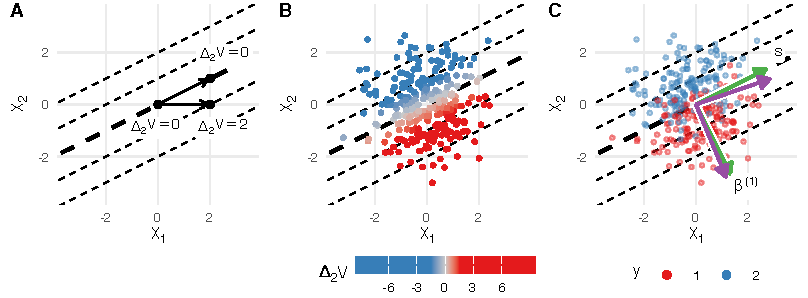
\includegraphics[width=\textwidth]{illustration}
    \caption{Illustration of the type-I and type-III initialization for $J = 2$ alternatives. In the type-I case, the axes show two regressors $X_1$ and $X_2$ of the first alternative with coefficient $\beta^{(1)} = \protect\begin{bmatrix} 1 & -2 \protect\end{bmatrix}^\top$, and the systematic utility of the second alternative is fixed at zero. In the type-III case, they show the values $X_1$ and $X_2$ of a single regressor for the two alternatives with coefficient $\beta^{(3)} = \protect\begin{bmatrix} 1 & 2 \protect\end{bmatrix}^\top$. Both cases yield the same utility difference $\Delta_2 V = V_1 - V_2$, which is constant along the dashed lines. These are orthogonal to $\beta^{(1)}$ and parallel to $s = \protect\begin{bmatrix} 1/\beta^{(3)}_1 & 1/\beta^{(3)}_2 \protect\end{bmatrix}^\top$. \textbf{A}: shifting a regressor combination along such a line leaves the utility difference unchanged. \textbf{B}: the utility difference across 300 simulated regressor combinations. \textbf{C}: the resulting choices, together with the directions of $\beta^{(1)}$ and $s$, in green for the true values and in purple for the estimates.}
    \label{fig:illustration}
\end{figure}

\subsection{Type-I coefficients}\label{sec:type1}

Consider first the model $U_{n,t} = X^{(1)}_{n,t} \beta^{(1)} + \epsilon_{n,t}$ where only type-I regressors are present. For given data, let $\tilde{\bm{X}} \in \R^{NTJ\times P_I}$ and $\tilde{\bm{y}}^d \in \R^{NTJ}$ denote the row-wise stacks of the centered design matrices and the centered dummy-encoded choices, where centering subtracts the overall sample means (for $\bm{X}$ column-wise), and consider the OLS estimate
%
\begin{align}
    \label{eq:ols}
    \hat{\alpha} = (\tilde{\bm{X}}^\top \tilde{\bm{X}})^{-1} \tilde{\bm{X}}^\top \tilde{\bm{y}}^d
\end{align}
%
of the linear probability model. Under the following conditions, $\hat{\alpha}/\norm{\hat{\alpha}}$ consistently estimates $\beta^{(1)}/\norm{\beta^{(1)}}$.
If $\beta^{(1)}$ is normalized for the utility scale by fixing its first entry $\beta^{(1)}_1 \neq 0$, then $\hat{\alpha} / \hat{\alpha}_1 \cdot \beta^{(1)}_1$ consistently estimates $\beta^{(1)}$ under specific assumptions on $\bm{X}$:

\begin{assumption}\label{asm:type1reg} The rows $X^{(1)}_{n,t,1,\cdot}, \dots, X^{(1)}_{n,t,J,\cdot}$ of the design matrix are independent and identically normally distributed across alternatives, with positive definite covariance matrix $\Var(X^{(1)}_{n,t,j,\cdot})$.
\end{assumption}


\begin{theorem} \label{thm:type1}
Consider the random utility system for $J$ alternatives and $P_I$ alternative-constant coefficients connected to alternative-varying regressors, i.e.,
%
\begin{align*}
    V_{n,t} &= X^{(1)}_{n,t} \beta^{(1)} = \begin{bmatrix} X^{(1)}_{n,t,1,1} & \dots & X^{(1)}_{n,t,1,P_I} \\ \vdots & \ddots & \vdots \\ X^{(1)}_{n,t,J,1} & \dots & X^{(1)}_{n,t,J,P_I} \end{bmatrix} \begin{bmatrix} \beta_1^{(1)} \\ \vdots \\ \beta_{P_I}^{(1)} \end{bmatrix} \in \R^J, \\
    U_{n,t} &= V_{n,t} + \epsilon_{n,t}, \\
    y_{n,t} &= \argmax U_{n,t}.
\end{align*}
%
Let Assumptions~\asmstar{1}, \asmstar{2}, \ref{asm:rationality}, and
\ref{asm:type1reg} hold and assume that
%
\begin{description}
    \asmitem\label{asm:type1coef} $\beta^{(1)} = \begin{bmatrix} \beta^{(1)}_1 & \beta^{(1)}_{-1} \end{bmatrix}^\top \in \R^{P_I}$ with $P_I \geq 2$ and $\beta^{(1)}_1 \neq 0$, which is fixed for identification of the utility scale.
\end{description}
%
Further, for given choice data, let $\tilde{\bm{X}} \in \R^{NTJ\times P_I}$ and $\tilde{\bm{y}}^d \in \R^{NTJ}$ denote the row-wise stacks of the design matrices $X^{(1)}_{n,t}$ and of the dummy-encoded choices $y_{n,t}^d$ after subtracting their overall sample means, where $y_{n,t,j}^d = 1$ if and only if $y_{n,t} = j$, and let $\hat{\alpha} = (\tilde{\bm{X}}^\top \tilde{\bm{X}})^{-1} \tilde{\bm{X}}^\top \tilde{\bm{y}}^d$. Then $$\hat{\alpha} \,/\, \hat{\alpha}_1 \cdot \beta^{(1)}_1 \pto \beta^{(1)},$$ where $\pto$ denotes convergence in probability as $NT \to \infty$.
\end{theorem}

\begin{proof}
Let $\bm{X} \in \R^{NTJ\times P_I}$ and $\bm{y}^d\in\{0,1\}^{NTJ}$ denote row-wise stacks of $X^{(1)}_{n,t}$ and $y_{n,t}^d$. For arbitrary but fixed alternative $j = 1,\dots,J$, define the submatrices $\bm{X}_j = \begin{bmatrix} X_{j,1} & X_{j,-1}^*\end{bmatrix} \in \R^{NT\times P_I}$ and $\bm{y}_j^d\in\{0,1\}^{NT}$ that keep only every $j$-th row of $\bm{X}$ and $\bm{y}^d$, respectively. Without loss of generality, we can assume that $\beta^{(1)} = \begin{bmatrix} 1 & 0 & \dots & 0 \end{bmatrix}^\top$ and that the column $X_{j,1}$ is uncorrelated with the remaining columns. That is because, given $\beta^{(1)}$, we can reparameterize $\bm{X}_{j} \beta^{(1)} = (\bm{X}_{j} M) (M^{-1} \beta^{(1)})$, where $M = \begin{bmatrix} \beta^{(1)} & \beta^{(1)}_\perp \end{bmatrix} \in \R^{P_I \times P_I}$ with submatrix $\beta^{(1)}_\perp \in \R^{P_I \times (P_I-1)}$ such that ${\beta^{(1)}_\perp}^\top \beta^{(1)} = 0_{P_I - 1}$ and ${\beta^{(1)}_\perp}^\top \beta^{(1)}_\perp = I_{P_I - 1}$, hence,
%
$$
M^{-1}\beta^{(1)} = \begin{bmatrix} \left({\beta^{(1)}}^\top\beta^{(1)}\right)^{-1} {\beta^{(1)}}^\top \\  {\beta^{(1)}_\perp}^\top \end{bmatrix} \beta^{(1)} = \begin{bmatrix} 1 & 0 & \dots & 0 \end{bmatrix}^\top.
$$
%
In this representation, the first column $X_{j,1}$ is the systematic utility of alternative $j$. Note that the choice of the basis $\beta^{(1)}_\perp$ is not unique, and multiples of $X_{j,1}$ can be added to the columns of $X_{j,-1}^*$ without changing $M^{-1}\beta^{(1)}$. In particular, replace $X_{j,-1}^*$ by $X_{j,-1} = X_{j,-1}^* - X_{j,1} \Var(X_{j,1})^{-1} \Cov(X_{j,1}, X_{j,-1}^*)$, in which case
%
\begin{align*}
    \Cov(X_{j,1}, X_{j,-1}) &= \Cov(X_{j,1}, X_{j,-1}^*) - \Var(X_{j,1}) \Var(X_{j,1})^{-1} \Cov(X_{j,1}, X_{j,-1}^*) \\
    &= 0_{P_I - 1}^\top
\end{align*}
%
such that the columns of the reparameterized regressor matrix are uncorrelated.

Now consider fitting the linear probability model $$\bm{y}_{j}^d = a_j + X_{j,1} \alpha_1 + X_{j,-1} \alpha_{-1} + u_{j}$$ to the data. The intercept $a_j$ can be concentrated out, leading to $\bm{y}_{j}^d$ and $\bm{X}_{j}$ being centered, which in the following is denoted using tildes:
%
\begin{align}
\label{eq:type1ols}
\tilde{\bm{y}}_{j}^d = \tilde{X}_{j,1} \alpha_1 + \tilde{X}_{j,-1} \alpha_{-1} + u_{j}.
\end{align}
%
By the Frisch--Waugh--Lovell theorem \citep{Frisch1933}, the OLS estimate $\hat \alpha_{-1}$ for $\alpha_{-1}$ in \eqref{eq:type1ols} is identical to the OLS estimate for $\alpha_{-1}$ in
%
\begin{align*}
\tilde{\bm{y}}_{j}^{d,\pi} = \tilde{X}_{j,-1}^{\pi} \alpha_{-1} + u_{j}^\pi,
\end{align*}
%
where superscripts $\pi$ denote projection onto the orthogonal complement of $\tilde{X}_{j,1}$. Since $\Cov(X_{j,-1}, X_{j,1}) = \Cov(\tilde{X}_{j,-1}, \tilde{X}_{j,1}) = 0_{P_I - 1}$, $\tilde{X}_{j,-1}^{\pi} \pto \tilde{X}_{j,-1}$ and $\Cov(\tilde{X}_{j,-1}, \tilde{\bm{y}}_{j}^{d,\pi}) \pto \Cov(\tilde{X}_{j,-1}, \tilde{\bm{y}}_{j}^d)$, which implies
%
\begin{equation}
\begin{aligned}
\label{eq:type1olslimit}
\hat{\alpha}_{-1} &= \left( (\tilde{X}_{j,-1}^{\pi}) ^\top \tilde{X}_{j,-1}^{\pi} \right)^{-1} (\tilde{X}_{j,-1}^{\pi}) ^\top \tilde{\bm{y}}_{j}^{d,\pi} \\ &\pto \Var(\tilde{X}_{j,-1}^\pi)^{-1} \Cov(\tilde{X}_{j,-1}^\pi,\tilde{\bm{y}}_{j}^{d, \pi}) = \Var(\tilde{X}_{j,-1})^{-1} \Cov(\tilde{X}_{j,-1},\tilde{\bm{y}}_{j}^d) \end{aligned}
\end{equation}
%
as $NT \to \infty$. Since $\beta^{(1)} = \begin{bmatrix} 1 & 0 & \dots & 0 \end{bmatrix}^\top$ and the rows of $X^{(1)}_{n,t}$ are independent across alternatives by Assumption~\ref{asm:type1reg}, the choice probabilities depend on the regressors of alternative $j$ only through $X_{j,1}$, hence $\tilde{\bm{y}}^d_{j}$ and $\tilde{X}_{j,-1}$ are conditionally independent given $\tilde{X}_{j,1}$, which implies
%
\begin{equation}
\begin{aligned}
\label{eq:type1olscovcalc}
\Cov(\tilde X_{j,-1},\tilde{\bm{y}}^d_{j}) &= \E(\tilde X_{j,-1}\tilde{\bm{y}}^d_{j}) = \E\left(\E(\tilde X_{j,-1}\tilde{\bm{y}}^d_{j} \mid \tilde{X}_{j,1})\right) \\ &= \E\left(\E(\tilde X_{j,-1} \mid \tilde{X}_{j,1}) \E(\tilde{\bm{y}}^d_{j} \mid \tilde{X}_{j,1})\right)
\end{aligned}
\end{equation}
%
by the law of iterated expectation. By Assumption~\ref{asm:type1reg}, $\tilde{X}_{j,-1}$ and $\tilde{X}_{j,1}$ are jointly normally distributed and uncorrelated, so that $\E(\tilde X_{j,-1} \mid \tilde{X}_{j,1}) = 0_{P_I - 1}$, hence \eqref{eq:type1olscovcalc} implies $\Cov(\tilde X_{j,-1},\tilde{\bm{y}}^d_{j}) = 0_{P_I - 1}$ and hence \eqref{eq:type1olslimit} yields $\hat{\alpha}_{-1} \pto 0_{P_I - 1}$.

By contrast, $\hat{\alpha}_1 \pto \Cov(\tilde{X}_{j,1}, \tilde{\bm{y}}_j^d) \Var(\tilde{X}_{j,1})^{-1} \neq 0$ since $\beta^{(1)}_1 \neq 0$ by Assumption~\ref{asm:type1coef}. It follows that $\beta^{(1)}$ can be consistently estimated using $\hat \alpha / \hat{\alpha}_1 \cdot \beta^{(1)}_1$. The above steps can analogously be conducted for every $j = 1,\dots,J$, which yields $J$ consistent estimators, with the average being again consistent.
\end{proof}

The coefficients $\beta^{(1)}$ are identified up to a multiplicative constant only, so that other normalization schemes than $\hat{\alpha} / \hat{\alpha}_1 \cdot \beta^{(1)}_1$ can be used, for instance $\norm{\beta^{(1)}} = 1$. For numerical reasons, our implementation normalizes the estimate to unit Euclidean length: the division by $\hat{\alpha}_1$ is unstable when $\hat{\alpha}_1$ is close to zero, and it presumes that the utility scale is fixed through $\beta^{(1)}_1$, whereas the scale can as well be fixed through an element of the error covariance matrix.

Algorithm~\ref{alg:type1init} states the procedure for arbitrary $J \geq 2$ and $P_I \geq 1$. Since it relies only on a few matrix operations, $\hat{\alpha}$ in \eqref{eq:ols} is obtained in a fraction of a second even for large samples. We make the following remarks:
%
\begin{itemize}
    \item Normality in Assumption~\ref{asm:type1reg} is sufficient but not necessary. The proof only uses that the regressor directions which are uncorrelated with the systematic utility have conditional mean zero given the systematic utility.
    \item The arguments do not invoke the specific form of $F_\epsilon$. Consistency therefore also holds for the multinomial logit specification; for arbitrary error covariances $\Var(\epsilon_{n,t}) = \Sigma$, even heteroskedastic ones; in the presence of ASCs; and in the presence of additional type-II or type-III regressors, provided these enter utility linearly and are independent of the type-I regressors.
\end{itemize}

\begin{algorithm}[htbp]
    \caption{Initial estimates for type-I coefficients.}
    \label{alg:type1init}
    \begin{algorithmic}[1]
        \REQUIRE choice data $\bm{X} \in \R^{NTJ \times P_I}$, $\bm{y} \in \{1,\dots,J\}^{NT}$
        \STATE transform $\bm{y}$ to dummy-encoded choices $\bm{y}^d \in \{0,1\}^{NTJ}$
        \STATE center $\tilde{\bm{X}} \leftarrow \bm{X} - 1_{NTJ} \bar{x}^\top$ and $\tilde{\bm{y}}^d \leftarrow \bm{y}^d - 1_{NTJ} \bar{y}^d$, with means $\bar{x}$ of the columns of $\bm{X}$ and $\bar{y}^d$ of $\bm{y}^d$
        \STATE calculate OLS estimate $\hat{\alpha} \leftarrow (\tilde{\bm{X}}^\top \tilde{\bm{X}})^{-1} \tilde{\bm{X}}^\top \tilde{\bm{y}}^d$
        \STATE normalize $\widehat{\beta^{(1)}} \leftarrow \hat{\alpha} / \norm{\hat{\alpha}}$
        \ENSURE initial estimate $\widehat{\beta^{(1)}}$ for the direction of $\beta^{(1)}$
    \end{algorithmic}
\end{algorithm}

While the assumptions of the theorem appear overly strong, the proof
reveals that the main fact used is that the conditional choice probability
of the $j$-th alternative only depends on variation of the regressor in
the direction $\beta^{(1)}/ \norm{\beta^{(1)}}$, while variation in its orthogonal complement
does not change the probability, cf.\ Figure~\ref{fig:illustration}.
The key here is $\E\left( \tilde X_{j,-1}\tilde{\bm{y}}^d_{j} \right) = 0$, for which the theorem provides one set of sufficient conditions.
This is picked up by the OLS fit.

Additionally one obtains

\begin{align*}
\Cov(\tilde X_{j,-1},\tilde{\bm{y}}^d_{j}) &= \E\left(\E(\tilde X_{j,-1} \mid \tilde{X}_{j,1}) \E(\tilde{\bm{y}}^d_{j} \mid \tilde{X}_{j,1})\right) \\
&= \E\left(\E(\tilde X_{j,-1} \mid \tilde{X}_{j,1})  \tilde X_{j,1} \alpha  \right) \\
&\quad + \E\left(\E(\tilde X_{j,-1} \mid \tilde{X}_{j,1}) (\E(\tilde{\bm{y}}^d_{j}  \mid \tilde{X}_{j,1}) - \alpha \tilde X_{j,1}) \right) \\
&= \E\left(\tilde X_{j,-1} \tilde X_{j,1} \alpha  \right)
+ \E\left(\tilde X_{j,-1} (\E(\tilde{\bm{y}}^d_{j}  \mid \tilde{X}_{j,1}) - \alpha \tilde X_{j,1}) \right) \\
&= \E\left(\tilde X_{j,-1} (\E(\tilde{\bm{y}}^d_{j}  \mid \tilde{X}_{j,1}) - \alpha \tilde X_{j,1}) \right).
\end{align*}

Here $r(\tilde{X}_{j,1}) \coloneq (\E(\tilde{\bm{y}}^d_{j}  \mid \tilde{X}_{j,1}) - \alpha \tilde X_{j,1})$ is a function of $\tilde{X}_{j,1}$. For
$\alpha$ equaling the OLS estimator, it equals the residual
of the linear probability model estimate. Thus it typically
is small. $\tilde X_{j,-1}$ is uncorrelated with $\tilde{X}_{j,1}$ by construction. Thus its correlation with $r(\tilde{X}_{j,1})$ typically will be small, even if not zero.
This suggests that the initialization remains useful for more general regressors.

\subsection{Type-II coefficients}\label{sec:type2}

Next, we treat type-II regressors, which, in contrast to type-I regressors, do not vary across alternatives but instead are connected to alternative-specific coefficients. Consider first the presence of a single type-II regressor $x_{n,t} \in \R$, which can be represented by a utility system with $J$ type-I coefficients $\beta^{(2)} \in \R^J$ as
%
\begin{align}
    \label{eq:type2system}
    \begin{bmatrix} U_{n,t,1} \\ \vdots \\ U_{n,t,J} \end{bmatrix} = \begin{bmatrix} x_{n,t} & 0 & 0 \\ 0 & \ddots & 0 \\ 0 & 0 & x_{n,t} \end{bmatrix} \begin{bmatrix} \beta^{(2)}_1 \\ \vdots \\ \beta^{(2)}_J \end{bmatrix} + \begin{bmatrix} \epsilon_{n,t,1} \\ \vdots \\ \epsilon_{n,t,J} \end{bmatrix}
    = x_{n,t} \begin{bmatrix} \beta^{(2)}_1 \\ \vdots \\ \beta^{(2)}_J \end{bmatrix} + \begin{bmatrix} \epsilon_{n,t,1} \\ \vdots \\ \epsilon_{n,t,J} \end{bmatrix}
    ,
\end{align}
%
with $\beta^{(2)}_1 = 0$ fixed for identifiability. This representation makes it clear that each alternative's regressor vector has only a single non-zero coordinate, hence the positive definite within-alternative covariance required in Assumption~\ref{asm:type1reg} is violated, and the arguments of Theorem~\ref{thm:type1} do not apply.

Instead, assume that a sample is given with fixed regressor value $x_{n,t} = x^\ast \neq 0$ and that $F_\epsilon$ is known. Then the choice probabilities are a known function $p(s)$ of the systematic utilities $s^\ast = \beta^{(2)}_{-1} x^\ast$ of alternatives $2,\dots,J$, and we can compute the minimizer
%
\begin{align}
    \label{eq:matching}
    \hat{s}(x^*) = \argmin_{s^* \in \R^{J-1}} \left\lVert \hat{f}(x^*) - p(s^*) \right\rVert_2
\end{align}
%
of the Euclidean distance between the observed (local to $x^*$) choice frequencies $\hat{f}(x^*)$ derived from $\bm{y}$ and the predicted choice probabilities. Then $\hat{s}(x^\ast) / x^\ast$ estimates $\beta^{(2)}_{-1}$. If $x_{n,t}$ takes a small number $K$ of different values, \eqref{eq:matching} analogously yields $K$ estimates, with the average being again consistent.\footnote{Note that constant $x^\ast = 1$ is equivalent to ASCs, while a finite number of values typically occurs for decider-specific characteristics like household size or age.} If the regressor is continuous, consistency can be achieved by localization, for example by $k$-means clustering \citep{Hartigan1979}, provided the number of observations in each cluster grows without bound and the within-cluster variances approach zero.


\begin{theorem} \label{thm:type2}
Consider the random utility system for $J$ alternatives and alternative-varying coefficients connected to alternative-constant regressors, i.e.,
%
\begin{align*}
    U_{n,t} = x_{n,t} \beta^{(2)}
    + \epsilon_{n,t} \in \R^J,
\end{align*}
%
with coefficients $\beta^{(2)} \in \R^J$, $\beta^{(2)}_1 = 0$ fixed for identifiability, and systematic utilities $s(x,\beta_{-1}^{(2)}) = x \, \beta_{-1}^{(2)} \in \R^{J-1}$ of alternatives $2, \dots, J$. For a given sample, let $C_1, \dots, C_K$ be $K$ disjoint local neighborhoods of the regressors with centers $c_1, \dots, c_K$. Let Assumptions~\asmstar{1}, \asmstar{2}, and \ref{asm:rationality} hold and assume that
%
\begin{description}
    \asmitem\label{asm:type2moment} $\E(\lvert x_{n,t} \rvert^2) < \infty$ and $\Pr(\lvert x_{n,t} \rvert > \tau) > 0$ for some $\tau>0$,
    \asmitem\label{asm:type2map} $p_{-1}(s) = \E(y^d_{n,t,-1} \mid s(x_{n,t}, \beta_{-1}^{(2)}) = s)$ is continuously differentiable on $\{s(x, \beta_{-1}^{(2)}) \mid |x| > \tau\}$ with non-singular Jacobian at $s(c_k, \beta_{-1}^{(2)})$ for each $k=1,\dots,K$,
    \asmitem\label{asm:type2cluster} $\Var(x_{C_k}) = \lvert C_k \rvert^{-1} \sum_{C_k} (x_{n,t} - c_k)^2 \to 0$, $\lvert C_k \rvert \to \infty$, and $\lvert c_k \rvert > \tau$, for $NT \to \infty$.
\end{description}
%
For each $k = 1,\dots,K$, let $\hat f_{k,-1} = \lvert C_k \rvert^{-1} \sum_{C_k} y_{n,t,-1}^d$ and $\hat{s}_k = p_{-1}^{-1}(\hat{f}_{k,-1})$. Then $$\hat{s}_k \,/\, c_k \pto \beta_{-1}^{(2)}.$$
\end{theorem}

\begin{proof}
Assumption~\ref{asm:type2moment} ensures that neighborhoods with the properties required in Assumption~\ref{asm:type2cluster} exist. Since $\lvert C_k \rvert \to \infty$ by Assumption~\ref{asm:type2cluster}, the law of large numbers yields
%
\begin{align*}
&\hat{f}_{k,-1} - \lvert C_k \rvert^{-1} \sum_{C_k} \E(y_{n,t,-1}^d \mid x_{n,t}) \\
&\qquad = \hat{f}_{k,-1} - \lvert C_k \rvert^{-1} \sum_{C_k} p_{-1}(s(x_{n,t}, \beta_{-1}^{(2)})) \pto 0_{J-1}.
\end{align*}
%
Since the composition $p_{-1} \circ s$ is continuous at $c_k$ and $\Var(x_{C_k}) \to 0$ by Assumption~\ref{asm:type2cluster}, we also have
%
\begin{align*}
     \lvert C_k \rvert^{-1} \sum_{C_k} p_{-1}(s(x_{n,t}, \beta_{-1}^{(2)})) \pto p_{-1}(s(c_k, \beta_{-1}^{(2)})),
\end{align*}
%
which implies $\hat{f}_{k,-1} \pto p_{-1}(s(c_k, \beta_{-1}^{(2)}))$ as $NT \to \infty$. By Assumption~\ref{asm:type2map}, the inverse function theorem guarantees the existence of a local inverse $p_{-1}^{-1}$ with $$\hat{s}_k = p_{-1}^{-1}(\hat{f}_{k,-1}) \pto s_{k} = s(c_k, \beta_{-1}^{(2)}).$$ Since $s_{k,j}=\beta^{(2)}_j\,c_k$ and $\lvert c_k \rvert > \tau > 0$ by Assumption~\ref{asm:type2cluster},
%
\begin{align*}
    \hat{\beta}_j^{(2)} = \frac{\hat{s}_{k,j}}{c_k} \pto \frac{s_{k,j}}{c_k} = \beta^{(2)}_j, \quad j = 2,\dots,J.
\end{align*}
%
The above steps can analogously be conducted for every $k = 1,\dots,K$, which yields $K$ consistent estimators, with the average being again consistent.
\end{proof}

Algorithm~\ref{alg:type2initsingle} summarizes the procedure. In our implementation, the number of clusters is at most $K = 10$ and is reduced until every cluster contains at least $10\%$ of the observations, and clusters with center $\lvert c_k \rvert \leq 0.001$ or a non-convergent minimization in line~\ref{algline:type2opt} are discarded. The per-cluster estimates are normalized to unit length and averaged with weights proportional to the cluster sizes. For $J = 2$, a type-II regressor is equivalent to a type-I regressor that takes the value zero for the first alternative, and it is treated as such. We note:
%
\begin{itemize}
    \item Since the probability map $p_{-1}$ is invoked, the theorem assumes that $F_\epsilon$ is specified correctly. If $\Sigma$ is unknown, or the data generating process (DGP) is not MNP, the MNP probabilities with $\Sigma = I_J$ can still serve as an approximation of the true probability map.
    \item The optimization step in line~\ref{algline:type2opt} of Algorithm~\ref{alg:type2initsingle} again requires numerical optimization. It is, however, much cheaper than full MLE, since the objective is only $(J-1)$-dimensional and each evaluation requires only $J$ Gaussian CDFs of dimension $J-1$.
    \item The clustering step can be replaced by a kernel estimator. Then the bandwidth choice replaces the choice of the number of clusters $K$.
    \item If multiple type-II regressors are present, the same steps can be conducted separately for each regressor after orthogonalization, see Algorithm~\ref{alg:type2init}.
\end{itemize}

\begin{algorithm}[htb]
  \caption{Initial estimates for a single type-II coefficient.}
  \label{alg:type2initsingle}
  \begin{algorithmic}[1]
    \REQUIRE choice data $\bm{X} \in \R^{NT}$, $\bm{y} \in \{1,\dots,J\}^{NT}$; fixed value $\beta^{(2)}_{1} = 0$; maximal number of clusters $K$
    \STATE transform $\bm{y}$ to dummy-encoded choices $\bm{y}^d \in \{0,1\}^{NT \times J}$ (row-wise)
    \STATE localize $\bm{X}$ using $k$-means with at most $K$ clusters, reducing $K$ until every cluster holds at least $10\%$ of the observations; obtain cluster allocations $C_1,\dots,C_K$ and centers $c_1, \dots, c_K$
    \FOR{$k = 1,\dots,K$ with $\lvert c_k \rvert > 0.001$}
      \STATE $\hat{f}_k \leftarrow \bm{y}_{C_k}^{d\top} 1_{\lvert C_k \rvert}\lvert C_k \rvert^{-1}$
      \STATE $\hat{s}_k \leftarrow \underset{s \in \R^{J-1}}{\argmin}\,\left\lVert \hat{f}_k - \begin{bmatrix} \Phi_{J-1}\left( -\Delta_{j} \begin{bmatrix} 0 \\ s \end{bmatrix} \,\middle|\, 0_{J-1}, \Delta_{j} I_{J} \Delta_{j}^\top \right) \end{bmatrix}_j \right\rVert_2$ \label{algline:type2opt}
      \STATE normalize $\widehat{{}^{k}_{}\beta_{-1}^{(2)}} \leftarrow (\hat{s}_k / c_k) \,/\, \norm{\hat{s}_k / c_k}$
    \ENDFOR
    \STATE calculate weighted average $\widehat{\beta_{-1}^{(2)}} \leftarrow \sum_k\, \lvert C_k \rvert\, \widehat{{}^{k}_{}\beta_{-1}^{(2)}} \,/\, \sum_k \lvert C_k \rvert$ over the retained clusters and normalize it to unit length
    \ENSURE initial estimate $\widehat{\beta_{-1}^{(2)}}$ for the direction of $\beta_{-1}^{(2)}$
  \end{algorithmic}
\end{algorithm}

\begin{algorithm}[htb]
  \caption{Initial estimates for multiple type-II coefficients.}
  \label{alg:type2init}
  \begin{algorithmic}[1]
    \REQUIRE choice data $\bm{X} \in \R^{NT \times P_{II}}$, $\bm{y} \in \{1,\dots,J\}^{NT}$
    \FOR{$p=1,\dots,P_{II}$}
      \STATE orthogonalize $\bm{X}_{p}$ with respect to $\bm{X}_{-p}$
      \STATE calculate $\widehat{\beta^{(2,p)}}$ via Algorithm~\ref{alg:type2initsingle}
    \ENDFOR
    \STATE transform $\bm{X}$, $\widehat{\beta^{(2)}} = \begin{bmatrix} \widehat{\beta^{(2,1)}} & \dots & \widehat{\beta^{(2,P_{II})}} \end{bmatrix}^\top$ into a type-I system ${\tilde{\bm{X}} = \bm{X} \widehat{\beta^{(2)}}}$ with one composite regressor per type-II regressor, which takes the value zero for the reference alternative
    \STATE obtain scale factors $\hat{\gamma} \in \R^{P_{II}}$ for $\bm{X} = \tilde{\bm{X}}$ via Algorithm~\ref{alg:type1init}
    \FOR{$p=1,\dots,P_{II}$}
      \STATE rescale $\widehat{\beta^{(2,p)}} \leftarrow \widehat{\beta^{(2,p)}} \cdot \hat{\gamma}_p$
    \ENDFOR
    \STATE normalize $\begin{bmatrix} \widehat{\beta^{(2,1)}} & \dots & \widehat{\beta^{(2,P_{II})}} \end{bmatrix}^\top$ to unit length
    \ENSURE initial estimate $\begin{bmatrix} \widehat{\beta^{(2,1)}} & \dots & \widehat{\beta^{(2,P_{II})}} \end{bmatrix}^\top$ for the direction of $\beta^{(2)}$
  \end{algorithmic}
\end{algorithm}

Note that this step ignores the existence of other type-I or type-III regressors. For the algorithms they are considered as part of the error term. This issue is discussed in more detail in Section~\ref{sec:mixed}.

\subsection{Type-III coefficients}\label{sec:type3}

Regressors of the third type vary across alternatives (as type-I) and are connected to alternative-specific coefficients (as type-II). Each type-III regressor can be expressed by $J$ type-I coefficients, analogous to \eqref{eq:type2system}, but with non-constant entries in the diagonal design matrix. This makes it clear that the regression approach of Section~\ref{sec:type1} is unsuitable for the same reason noted in Section~\ref{sec:type2}, while the method of choice frequency matching of Section~\ref{sec:type2} becomes infeasible due to the need for multi-dimensional localization. Instead, another model structure can be exploited.

Consider $V_{n,t,j} = X_{n,t,j} \beta^{(3)}_j$ for $j = 1,\dots,J$. Since $(X_{n,t,j} + c / \beta^{(3)}_j) \beta^{(3)}_j = V_{n,t,j} + c$ for any $c \in \R$, all systematic utilities shift by the same constant along the direction $s = \begin{bmatrix} 1/\beta^{(3)}_1 & \dots & 1/\beta^{(3)}_J \end{bmatrix}^\top$ in the regressor space, and utility differences remain unchanged, compare Figure~\ref{fig:illustration}. In a correctly specified model, the choice probabilities are therefore constant along this direction. For given data, this motivates identifying the direction along which the empirical covariance between dummy-encoded choices and regressors is approximately zero, which is spanned by the right singular vector of the covariance matrix associated with its smallest singular value. The element-wise inverse of this vector estimates the direction of $\beta^{(3)}$.

\begin{theorem} \label{thm:type3}
Consider the utilities $U_{n,t,j}=V_{n,t,j}+\epsilon_{n,t,j}$, $V_{n,t,j}=X_{n,t,j}\beta^{(3)}_j$, $j\in\{1,\dots,J\}$, with type-III coefficient $\beta^{(3)} = \begin{bmatrix}\beta^{(3)}_1&\dots&\beta^{(3)}_J\end{bmatrix}^\top \in \R^J$, $\norm{\beta^{(3)}}=1$ and $\beta^{(3)}_1>0$ for identification, and dummy-encoded choices $y^d_{n,t}$. Define $\tilde X_{n,t}=X_{n,t}-\E(X_{n,t})$, $\tilde y^d_{n,t}=y^d_{n,t}-\E(y^d_{n,t})$, and $p(x)=\E(\tilde y^d_{n,t}\mid \tilde X_{n,t}=x)$, where $X_{n,t}=\begin{bmatrix}X_{n,t,1} & \dots & X_{n,t,J}\end{bmatrix}^\top$. Let Assumptions~\asmstar{1}, \asmstar{2}, and \ref{asm:rationality} hold and assume that
%
\begin{description}
  \asmitemvar{\asmstar{\ref*{asm:type1coef}}}\label{asm:type3coef} $\beta^{(3)}_j \neq 0$ for all $j \in \{1,\dots,J\}$,
  \asmitemvar{\asmstar{\ref*{asm:type2moment}}}\label{asm:type3moment} $\E (\norm{X_{n,t}}^2) < \infty$,
  \asmitem\label{asm:type3proj} For $s\in\R^J$ with $s_j=1/\beta^{(3)}_j$, there exists a linear projection $\Pi_s$ onto the space spanned by $s$ such that, with $\Pi_\perp = I_J-\Pi_s$, one has the decomposition
  $\tilde X_{n,t}=\Pi_s\tilde X_{n,t}+\Pi_\perp \tilde X_{n,t}$ where  $\Pi_s\tilde X_{n,t}$ is independent of $\Pi_\perp \tilde X_{n,t}$,
  \asmitem\label{asm:type3rank} $M = \E ( \tilde y^d_{n,t} \tilde X_{n,t}^\top ) \in\R^{J\times J}$ has rank $J-1$.
\end{description}
%
Let $\widehat{M} = (NT)^{-1} \sum_{n,t} \tilde y^d_{n,t}\,(\tilde X_{n,t})^\top$, $\hat v$ be the unit right singular vector of $\widehat{M}$ associated with its smallest singular value such that $\hat v_1 > 0$, and
$\hat\beta = \begin{bmatrix} \hat v_1^{-1} & \dots & \hat v_J^{-1} \end{bmatrix}^\top$. Then $$ \hat{\beta} \, / \, \norm{\hat{\beta}} \pto \beta^{(3)}.$$
\end{theorem}

\begin{proof}
Note that $s$ is well defined by Assumption~\ref{asm:type3coef},
and that in this setting, $$(X_{n,t,j}+c\,s_j)\,\beta^{(3)}_j=V_{n,t,j}+c \quad \text{for all}~c \in \R,\ j\in\{1,\dots,J\}.$$ Therefore it holds that $p(x)=p(\Pi_\perp x)$ for all $x\in\R^J$, hence $\tilde{y}^d_{n,t}$ is independent of $\Pi_s \tilde{X}_{n,t}$ given $\Pi_\perp \tilde{X}_{n,t}$.
Since $$\E\left((\Pi_s \tilde{X}_{n,t})^\top \mid \Pi_\perp \tilde{X}_{n,t}\right) = \E \left((\Pi_s \tilde{X}_{n,t})^\top \right) = 0_{J}$$
by Assumption~\ref{asm:type3proj}
and by the law of iterated expectation,
%
\begin{align*}
    M \Pi_s &= \E \left(\tilde{y}_{n,t}^d (\Pi_s \tilde{X}_{n,t})^\top \right) = \E \left( \E(\tilde{y}_{n,t}^d (\Pi_s \tilde{X}_{n,t})^\top \mid \Pi_\perp \tilde{X}_{n,t}) \right) \\
    &= \E \left( \E(\tilde{y}_{n,t}^d \mid \Pi_\perp \tilde{X}_{n,t}) \E((\Pi_s \tilde{X}_{n,t})^\top \mid \Pi_\perp \tilde{X}_{n,t}) \right) = 0_{J \times J}.
\end{align*}
%
Since $\Pi_s s = s$, we have $M s = 0_{J}$, hence $s$ lies in the kernel of $M$. As $M$ has rank $J - 1$ by Assumption~\ref{asm:type3rank}, $s$ spans the kernel of $M$.

By Assumption~\ref{asm:type3moment}
and the law of large numbers, $\widehat{M} \pto M$ as $NT\to\infty$. Let $\hat v$ be the unit right singular vector of $\widehat{M}$ associated with its smallest singular value such that $\hat v_1 > 0$, then $\hat v \pto s\, /\, \norm{s}$. Let
$\hat\beta = \begin{bmatrix} \hat v_1^{-1} & \dots & \hat v_J^{-1} \end{bmatrix}^\top$, then $$ \hat{\beta} \, / \, \norm{\hat{\beta}} \pto \beta^{(3)}.$$
\end{proof}

Algorithm~\ref{alg:type3init} summarizes the procedure, which only requires a singular value decomposition of a $J \times J$ matrix and hence is computed very fast. The singular vector $\hat v$ is determined up to its sign only, and so is $\hat{\beta}$. The theorem resolves this ambiguity through $\hat v_1 > 0$, which presumes that the sign of $\beta^{(3)}_1$ is known. The implementation instead infers the sign from the data. The diagonal element $\widehat{M}_{jj}$ is the empirical covariance between the regressor of alternative $j$ and the indicator of choosing alternative $j$. If $\beta^{(3)}_j > 0$, a larger value of this regressor raises the utility of alternative $j$ and thereby its choice probability, so that $M_{jj} > 0$, and if $\beta^{(3)}_j < 0$, then $M_{jj} < 0$. Under the true coefficients, $M_{jj} \beta^{(3)}_j$ is therefore positive for every $j$, and of the two candidates $\hat{\beta}$ and $-\hat{\beta}$ the implementation selects the one that satisfies $\sum_j \widehat{M}_{jj} \hat{\beta}_j > 0$. We note:
%
\begin{itemize}
    \item Independence between $\Pi_s \tilde{X}_{n,t}$ and $\Pi_\perp \tilde{X}_{n,t}$
    in Assumption~\ref{asm:type3proj}
    is given, for example, if $X_{n,t}$ is jointly normally distributed.
    \item The rank condition
    in Assumption~\ref{asm:type3rank}
    is required to uniquely identify the direction $v$. It is fulfilled if the choice probabilities vary with the regressors apart from the direction $s$.
    \item The particular form of the probability map $p(\cdot)$ is not invoked, therefore consistency is robust to the specification of $F_\epsilon$.
    \item If multiple type-III regressors are present, the same steps can be conducted separately after partialling out the other type-III regressors, see Section~\ref{sec:mixed}.
\end{itemize}

\begin{algorithm}[htbp]
  \caption{Initial estimates for type-III coefficients.}
  \label{alg:type3init}
  \begin{algorithmic}[1]
    \REQUIRE choice data $\bm{X} \in \R^{NT \times JP_{III}}$, $\bm{y} \in \{1,\dots,J\}^{NT}$
    \STATE transform $\bm{y}$ to dummy-encoded choices $\bm{y}^d \in \{0,1\}^{NT \times J}$ (row-wise)
      \FOR{$p = 1,\dots,P_{III}$}
        \IF{$P_{III} > 1$}
        \STATE orthogonalize $\bm{X}_{\cdot, p}$ and $\bm{y}^d$ with respect to $\bm{X}_{\cdot, -p}$
        \ENDIF
        \STATE $\widehat{M} \leftarrow \Cov(\bm{y}^d,\ \bm{X}_{\cdot, p})$
        \STATE compute singular value decomposition $\widehat{M} = UDV^\top$
        \STATE identify $\hat v \in \R^J$ as the unit right singular vector of $\widehat{M}$ associated with its smallest singular value
        \STATE $\widehat{\beta^{(3,p)}} \leftarrow \hat v^{-1} / \norm{\hat v^{-1}}$ ($\hat v^{-1}$ denotes the element-wise inverse of $\hat v$), with the sign of $\hat v$ chosen such that $\sum_j \widehat{M}_{jj} \widehat{\beta^{(3,p)}_j} > 0$
      \ENDFOR
      \IF{$P_{III} > 1$}
      \STATE transform $\bm{X}$, $\widehat{\beta^{(3)}} = \begin{bmatrix} \widehat{\beta^{(3,1)}} & \dots & \widehat{\beta^{(3,P_{III})}} \end{bmatrix}^\top$ into a type-I system ${\tilde{\bm{X}} = \bm{X} \widehat{\beta^{(3)}}}$
    \STATE obtain scale factors $\hat{\gamma} \in \R^{P_{III}}$ for $\bm{X} = \tilde{\bm{X}}$ via Algorithm~\ref{alg:type1init}
    \FOR{$p=1,\dots,P_{III}$}
      \STATE rescale $\widehat{\beta^{(3,p)}} \leftarrow \widehat{\beta^{(3,p)}} \cdot \hat{\gamma}_p$
    \ENDFOR
    \ENDIF
    \STATE normalize $\begin{bmatrix} \widehat{\beta^{(3,1)}} & \dots & \widehat{\beta^{(3,P_{III})}} \end{bmatrix}^\top$ to unit length
    \ENSURE initial estimate $\begin{bmatrix} \widehat{\beta^{(3,1)}} & \dots & \widehat{\beta^{(3,P_{III})}} \end{bmatrix}^\top$ for the direction of $\beta^{(3)}$
  \end{algorithmic}
\end{algorithm}

\subsection{Multiple regressor types}\label{sec:mixed}

If regressors of several types are present, or several type-II or type-III regressors, the estimators of Sections~\ref{sec:type1} to \ref{sec:type3} are applied after orthogonalization, following the idea of the Frisch--Waugh--Lovell theorem \citep{Frisch1933}. The group of type-I regressors is regressed on all remaining regressors, and each type-II and type-III regressor on all other regressors, and the estimators are applied to the residuals. For the type-I and type-III steps, the dummy-encoded choices are residualized in the same way; for the type-II step, the choices are kept unchanged to preserve proper choice frequencies.

Each of the resulting estimates is normalized and hence identified up to scale only, while the relative scales between the regressors are to be estimated. To determine them, each regressor block is collapsed into a single composite type-I regressor using its estimate, and the type-I system
%
\begin{multline}
    \label{eq:commonscale}
    U_{n,t} = \Bigl[ X^{(1)}_{n,t} \quad X^{(2)}_{n,t,1} \widehat{\beta^{(2,1)}} \quad \dots \quad X^{(2)}_{n,t,P_{II}} \widehat{\beta^{(2,P_{II})}} \\
    X^{(3)}_{n,t,1} \widehat{\beta^{(3,1)}} \quad \dots \quad X^{(3)}_{n,t,P_{III}} \widehat{\beta^{(3,P_{III})}} \Bigr] \gamma + \epsilon_{n,t}
\end{multline}
%
is estimated by OLS after centering the composite regressors and the dummy-encoded choices within each choice occasion, where $X^{(2)}_{n,t,p}$ and $X^{(3)}_{n,t,p}$ denote the $J \times (J-1)$ and $J \times J$ design blocks of the $p$-th type-II and type-III regressor, respectively, and the type-II block is completed by a zero row for the reference alternative. The estimate $\hat{\gamma}$ of $\gamma$ in \eqref{eq:commonscale} provides the type-I coefficients together with a scale factor for each type-II and type-III block, and the resulting coefficient vector is again normalized to unit length. Algorithms~\ref{alg:type2init} and \ref{alg:type3init} contain the corresponding steps for multiple type-II and type-III regressors.

\subsection{Covariance matrices}\label{sec:covariance}

In the second step, initial values for $\tilde{\Sigma} = \Delta_1 \Sigma \Delta_1^\top$ and $\Omega$ are derived conditional on the coefficient estimate $\hat{b}$ from the first step via Gibbs sampling, computing sample means over a small number $R$ of iterations. The sampler is the data augmentation scheme for Bayesian probit models \citep{Albert1993, McCulloch1994}, where $b$ is kept fixed at $\hat{b}$ and not updated. Let $\tilde{U}_{n,t} = \Delta_1 U_{n,t}$ and $\tilde{X}_{n,t} = \Delta_1 X_{n,t}$ denote utilities and regressors differenced with respect to the first alternative. Each iteration consists of the following conditional draws:
%
\begin{enumerate}
    \item For each $n$ and $t$, the latent utility $\tilde{U}_{n,t}$ is drawn from $\Normal{J-1}{\tilde{X}_{n,t} \beta_n, \tilde{\Sigma}}$ truncated to the region consistent with the observed choice $y_{n,t}$.
    \item $\tilde{\Sigma}$ is drawn from its inverse Wishart conditional posterior
    %
    \begin{align*}
        \IW{J-1}{J + 1 + NT,\ I_{J-1} + \sum_{n,t} (\tilde{U}_{n,t} - \tilde{X}_{n,t} \beta_n)(\tilde{U}_{n,t} - \tilde{X}_{n,t} \beta_n)^\top},
    \end{align*}
    %
    which corresponds to the prior $\IW{J-1}{J+1, I_{J-1}}$.
    \item If $O$ coefficients are connected to random effects, $\Omega_{\Oset,\Oset}$ is drawn from
    %
    \begin{align*}
        \IW{O}{O + 2 + N,\ I_{O} + \sum_{n} (\beta_{n} - \hat{b})_{\Oset} (\beta_{n} - \hat{b})_{\Oset}^\top},
    \end{align*}
    %
    where the subscript $\Oset$ selects the random components, and subsequently each $\beta_{n,\Oset}$ is drawn from its Gaussian conditional posterior with prior mean $\hat{b}_{\Oset}$ and prior covariance $\Omega_{\Oset,\Oset}$, given $\tilde{U}_{n,\cdot}$ and $\tilde{\Sigma}$.
    If $O = 0$, then $\beta_n = \hat{b}$ for all $n$.
\end{enumerate}
\begin{algorithm}[htbp]
  \caption{Initial estimates for $\tilde{\Sigma} = \Delta_1 \Sigma \Delta_1^\top$ and $\Omega$.}
  \label{alg:covinit}
  \begin{algorithmic}[1]
    \REQUIRE choice data $\bm{X}$, $\bm{y}$; coefficient estimate $\hat{b}$; positions $\Oset$ of the $O$ random coefficients; number of iterations $R$; burn-in $B$
    \STATE difference $\bm{X}$ and the dummy-encoded choices $\bm{y}^d$ with respect to the first alternative, $\tilde{X}_{n,t} \leftarrow \Delta_1 X_{n,t}$, $\tilde{U}_{n,t} \leftarrow \Delta_1 y^d_{n,t}$
    \STATE set $\tilde{\Sigma} \leftarrow I_{J-1}$ and $\beta_n \leftarrow \hat{b}$ for $n = 1,\dots,N$
    \FOR{$i = 1,\dots,R$}
      \STATE draw $\tilde{U}_{n,t}$ from $\Normal{J-1}{\tilde{X}_{n,t} \beta_n, \tilde{\Sigma}}$ truncated to the region consistent with $y_{n,t}$, for all $n, t$
      \STATE draw $\tilde{\Sigma}$ from $\mathcal{IW}_{J-1}\bigl(J + 1 + NT,$\\ \hspace*{1.5em}$I_{J-1} + \sum_{n,t} (\tilde{U}_{n,t} - \tilde{X}_{n,t} \beta_n)(\tilde{U}_{n,t} - \tilde{X}_{n,t} \beta_n)^\top\bigr)$
      \IF{$O > 0$}
        \STATE draw $\Omega_{\Oset,\Oset}$ from $\mathcal{IW}_{O}\bigl(O + 2 + N, I_{O} + \sum_{n} (\beta_{n} - \hat{b})_{\Oset} (\beta_{n} - \hat{b})_{\Oset}^\top\bigr)$
        \STATE draw $\beta_{n,\Oset}$ from its Gaussian conditional posterior with prior $\Normal{O}{\hat{b}_{\Oset}, \Omega_{\Oset,\Oset}}$ given $\tilde{U}_{n,\cdot}$ and $\tilde{\Sigma}$, and set $\beta_{n,-\Oset} \leftarrow \hat{b}_{-\Oset}$, for ${n = 1,\dots,N}$
      \ENDIF
      \IF{$i > B$}
        \STATE store $\tilde{\Sigma}$ and $\Omega_{\Oset,\Oset}$
      \ENDIF
    \ENDFOR
    \STATE compute $\widehat{\tilde{\Sigma}}$ and $\widehat{\Omega_{\Oset,\Oset}}$ as the averages over the stored draws
    \ENSURE initial estimates $\vech(\chol(\widehat{\tilde{\Sigma}}))$ and $\vech(\chol(\widehat{\Omega_{\Oset,\Oset}}))$
  \end{algorithmic}
\end{algorithm}
%
The sampler is initialized at $\tilde{\Sigma} = I_{J-1}$, $\beta_n = \hat{b}$, and $\tilde{U}_{n,t} = \Delta_1 y^d_{n,t}$, aiming to speed up convergence. After a burn-in period of $B = R/2$ iterations, $\tilde{\Sigma}$ and $\Omega_{\Oset,\Oset}$ are estimated by the averages of the retained draws, and their Cholesky roots complete $\theta^{(0)}$, see Algorithm~\ref{alg:covinit}. We use $R = 200$ iterations and at most $N_{\max} = 1{,}000$ deciders. The purpose of this step is to provide approximate values for the covariance parameters at low computational cost, and simulations reported in \citet[Appendix C]{Oelschlaeger2026} indicate that the resulting Euclidean distances to the true parameters are small relative to random or identity initializations.

\section{Simulation Study}\label{sec:simulation}

\subsection{Design}

We evaluate the numerical benefits of the proposed initialization in six simulation scenarios, which are summarized in Table~\ref{tab:scenarios}. Scenarios S1 to S4 are cross-sectional with $N = 5{,}000$ deciders, $J = 5$ alternatives, and fixed coefficients of a single type (S1 to S3) or of all three types (S4). Scenarios S5 and S6 are panel settings with $N = 200$ deciders in $T = 10$ choice occasions and correlated Gaussian random effects.
The scenarios contain between $q=19$ (S1) and $q=39$ (S4) parameters.
In each replication, the regressor values and the DGP parameters $\theta_\text{DGP}$ are drawn independently from standard normal distributions, and choices are generated from the nMMNP model with unrestricted covariance matrices $\tilde{\Sigma}$ and $\Omega$. The utility level is fixed by expressing utilities relative to the first alternative, the utility scale by $\tilde{\Sigma}_{1,1} = [\Delta_1 \Sigma \Delta_1^\top]_{1,1} = 1$.

\begin{table}[htb]
    \centering
    \caption{Simulation scenarios.}
    \label{tab:scenarios}
    \resizebox{\textwidth}{!}{\input{sim_scenarios}}
\end{table}

Models are fitted with the same specification as the DGP by minimizing the negative log-likelihood function (S1 to S4) or, in S5 and S6, the negative logarithm of the pairwise CML function, which uses \eqref{eq:cml} in place of \eqref{eq:prob} in \eqref{eq:lik}. We use the approximation of the Gaussian CDF by \citet{Solow1990} and \citet{Joe1995} and analytical gradients as implemented in Rprobit \citep{Rprobit}.\footnote{All computations reported in this paper, for the simulation study as well as for the application, were carried out on a machine with 16 virtual CPUs and 32 GiB of memory under Ubuntu 26.04 LTS, using R 4.5.2 with 15 parallel workers.} The optimizer is the Newton-type routine \texttt{stats::nlm()} of R \citep{R}, based on \citet{Dennis1983}, with iteration limit $1{,}000$ and gradient and step tolerances of $10^{-8}$. For each of 100 replications per scenario, optimization is performed on the same data with three initializations: random draws $\theta^{(0)} \sim \Normal{q}{0_q, I_q}$, the proposed strategy (Algorithms~\ref{alg:type1init} to \ref{alg:covinit}), and the DGP parameters $\theta^{(0)} = \theta_\text{DGP}$. Note that random draws and DGP parameters can be interpreted as the two extremes of knowledge about the maximum likelihood estimate prior to optimization. Note further that DGP parameters and regressors are sampled from standard normal distributions, hence this setting already represents a case in which random initialization from a standard normal distribution is expected to perform comparatively well.

For each initialization, we record the computation time, including the time for computing the initial values, the number of optimizer iterations, the relative Euclidean distance $\norm{\theta^{(0)}- \theta_\text{DGP}} / \norm{\theta_\text{DGP}}$ of the initial values, and the objective value at termination. Since the global maximizer is unknown, we classify an optimization as successful if its objective value at termination lies within five units of the best value attained by any of the three initializations on the same data set, and if the relative Euclidean distance of the estimate to $\theta_\text{DGP}$ does not exceed five. The second condition detects divergence into flat regions of the objective, where the parameter norm becomes unbounded while the objective value barely changes.

\subsection{Results}

Table~\ref{tab:initial} summarizes the quality of the initial values. The median computation time of the proposed initial values ranged between 7 and 22 seconds across the scenarios. Relative to random draws, the median Euclidean distance to the DGP parameters is reduced to between 37\% and 56\% in the six scenarios, and the gap between the objective value at the initial values and the best objective value at termination is reduced by a factor between 20 and 613. Both reductions are smallest in S2, which we attribute to the type-II procedure evaluating the probability map at $\Sigma = I_J$, while the error covariance matrix of the DGP is unrestricted.

\begin{figure}[htb]
    \centering
    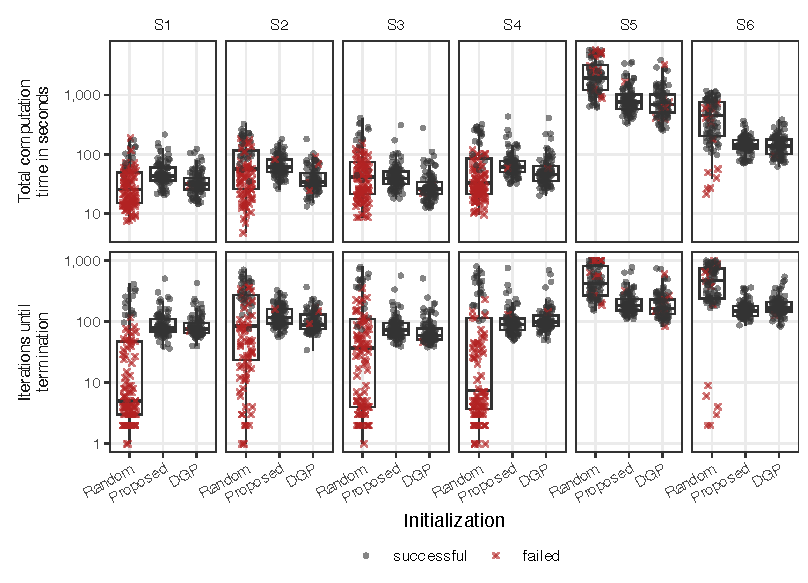
\includegraphics[width=\textwidth]{sim_optimization}
    \caption{Optimization outcomes. Total computation time, including initialization, and number of iterations until termination, 100 replications per scenario, logarithmic scale. Red crosses mark runs that were not successful.}
    \label{fig:optimization}
\end{figure}

\begin{table}[t]
    \centering
    \caption{Initial values. Medians over 100 replications of the computation time of the proposed initialization in seconds, the relative Euclidean distance $\norm{\theta^{(0)} - \theta_\text{DGP}} / \norm{\theta_\text{DGP}}$, and the gap between the objective value at $\theta^{(0)}$ and the best objective value at termination.}
    \label{tab:initial}
    \small
    \input{sim_initial}
\end{table}

\begin{table}[t]
    \centering
    \caption{Optimization outcomes. (a) Success rates over 100 replications. (b) Medians of the total computation time in seconds, including initialization. (c) Number of iterations among successful runs.}
    \label{tab:results}
    \resizebox{\textwidth}{!}{\input{sim_results}}
\end{table}

\begin{table}[t]
    \centering
    \caption{Reason for termination. Number of runs among 100 replications per scenario and initialization.}
    \label{tab:outcomes}
    \small
    \input{sim_outcomes}
\end{table}

Table~\ref{tab:results} and Figure~\ref{fig:optimization} summarize the optimization outcomes. Table~\ref{tab:outcomes} reports why the unsuccessful runs terminated, distinguishing four mutually exclusive cases that are assigned in the following order:
\begin{itemize}
    \item the estimate violates the distance criterion, because the norm of the parameter vector increased without bound while the objective value remained nearly constant (diverged);
    \item the optimizer terminated because the maximum number of iterations was reached before a convergence criterion was met (iteration limit);
    \item the optimizer terminated without meeting a convergence criterion, because its line search could not find a step that improves the objective value, which indicates a flat or numerically rough region of the objective (stalled);
    \item the optimizer met a convergence criterion at a stationary point whose objective value is below the best value (inferior optimum).
\end{itemize}
In the cross-sectional scenarios S1 to S4, random initialization was successful in only 15\% to 34\% of the replications, and in the panel scenarios S5 and S6 in 83\% and 85\%. In S1 to S4, most failures are diverged or stalled runs, which ended early, after a median of 4 to 37 iterations. This explains the low computation times and iteration counts of many randomly initialized runs in Figure~\ref{fig:optimization}. In the panel scenarios, most failures are divergences, and two runs in S5 terminated at the iteration limit. No run of the proposed or of the DGP initialization reached the iteration limit. Among the successful runs, random initialization required 2.0 to 4.5 times the median computation time and 2.1 to 5.7 times the median number of iterations of the proposed initialization. The proposed initialization was successful in 99\% to 100\% of the replications, compared to 91\% to 99\% for the DGP initialization. Its median computation time exceeded that of the DGP initialization by 7 to 63 seconds. Except in S5, most of this difference is the time needed for computing the initial values, which amounts to 7 to 22 seconds.

In the panel scenarios S5 and S6, where each function evaluation is considerably more expensive, the successful randomly initialized runs required a median of 1{,}779 and 485 seconds, respectively. The proposed initialization reduced these times to 761 and 145 seconds, with success rates of 99\% and 100\%, and required 9\% and 5\% more time than the DGP initialization. The number of iterations shows the same pattern: the proposed initialization required a median of 183 and 148 iterations, compared to 390 and 511 iterations for random initialization and 164 and 167 for the DGP parameters.

The proposed initialization failed in three replications overall, one each in S2, S4, and S5. In all three, the optimizer converged to a stationary point 6 to 12 units below the best value, and in the replication of S4 the DGP initialization ended at the same point. The DGP initialization failed in 20 replications overall, between 1 and 9 per scenario, each time ending 5 to 35 units below the best value that another initialization attained on the same data. In the nine such replications of S5, the proposed initialization attained the best value every time. Starting at the DGP parameters is thus no guarantee for reaching the global maximum in finite samples, where the maximum likelihood estimate differs from the DGP parameters. In summary, the proposed initialization attained the best objective value in 597 of the 600 replications, compared to 580 for the DGP initialization and 258 for random initialization, at a computation time close to that of the DGP initialization, which is infeasible in practice.

\section{Empirical Application}\label{sec:application}

We now demonstrate the initialization on an empirical data set, a panel with correlated random coefficients. The purpose is to show how it behaves on data that were not generated by the model and also do not satisfy all assumptions of the theorems above.

\begin{table}[htb]
    \centering
    \caption{Estimates $\hat{\theta}$ and proposed initial values $\theta^{(0)}$ in the empirical application. The parameters $O_1$ to $O_6$ are the free elements of the Cholesky root of the covariance matrix $\Omega$ of the random coefficients on price, operating cost, and acceleration time, the parameters $L_1$ and $L_2$ those of the error covariance matrix. HEV, PHEV, and BEV denote hybrid, plug-in hybrid, and battery electric powertrains, and the number after PHEV or BEV is the electric range in miles.}
    \label{tab:carsusest}
    \footnotesize
    \setlength{\tabcolsep}{3.5pt}
    \resizebox{\textwidth}{!}{\input{app_cars_us_estimates}}
\end{table}

We compare one optimization started at the proposed initial values with 100 optimizations started at random initial values $\theta^{(0)} \sim \Normal{q}{0_q, I_q}$, holding the optimizer and its termination criteria fixed at the settings of Section~\ref{sec:simulation}. Since the maximum likelihood estimate is unknown, we treat the largest objective value attained by any run as the reference and consider a run successful if its objective value is within two units of that reference. Since a failed run necessitates a restart, we compare the initializations by their cost per successful estimate, defined as the total number of iterations, or the total computation time, of all runs divided by the number of successful runs.

The scaling of the regressors affects this comparison, because it determines the magnitude of the coefficients, and thereby the distance between a standard normal draw and the optimum, as well as the conditioning of the optimization problem. We therefore standardize the continuous attributes by dividing them by their standard deviations and leave the indicators unscaled. As a result, the coefficients are of the same order of magnitude as the random initial values, which constitutes a favorable setting for random initialization and hence a conservative benchmark for the proposed initialization.

The data set is the US part of the conjoint survey of \citet{Helveston2015}, who study whether subsidies can drive the adoption of electric vehicles. In 2012, $N = 384$ respondents each chose $T = 15$ times between three vehicle profiles, giving 5{,}760 choices. A profile is described by its powertrain, namely conventional, hybrid, plug-in hybrid with 10, 20, or 40 miles of electric range, or battery electric with 75, 100, or 150 miles of range, by whether it can be charged rapidly, by its price in thousands of dollars, its operating cost in cents per mile, its acceleration time in seconds, and by the origin of its brand, namely German, American, Japanese, Chinese, or South Korean. The data are distributed with the R package logitr \citep{Helveston2023}.

\begin{figure}[t]
    \centering
    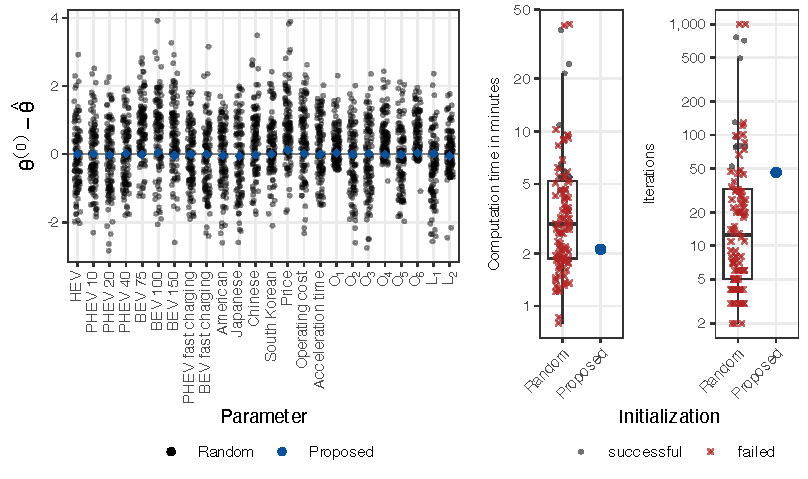
\includegraphics[width=\textwidth]{app_cars_us}
    \caption{Initialization and optimization results in the empirical application. Left: deviation of the initial values from the estimate, per parameter (labels as in Table~\ref{tab:carsusest}). Right: computation time in minutes, including initialization, and number of iterations until termination, on a logarithmic scale. Red crosses mark runs that were not successful.}
    \label{fig:carsus}
\end{figure}

All attributes enter with generic coefficients (type-I), coded as indicators against the conventional powertrain and the German brand as in the source. The model has no ASCs, as the ordering of the alternatives was chosen randomly. The coefficients of the price, the operating cost, and the acceleration time vary across respondents according to a correlated trivariate normal distribution. The error covariance matrix is left unrestricted, and the parameter vector has $q = 24$ entries, of which six belong to $\Omega$ and two to the error covariance matrix. Because the panel dimension makes the full likelihood expensive, we maximize the pairwise CML function, as in scenarios S5 and S6. Our specification differs from the source in two respects. \citet{Helveston2015} estimate a mixed logit model in the willingness-to-pay space, with a fixed price coefficient and independent normal random coefficients on all remaining attributes, and they weigh the respondents (using stratification weights) so that the age and income distributions match those of a reference survey. Our estimation is in the preference space and unweighted.

Figure~\ref{fig:carsus} summarizes the results. The proposed initialization attained the reference value $l(\hat{\theta}) = -4{,}531.67$ after 46 iterations, requiring 0.7 minutes for computing the initial values and 1.4 minutes for the optimization. Of the 100 random initializations, 10 attained the reference value, after a median of 88 iterations, and all successful runs terminated at the same estimate. The remaining 90 runs terminated at least 314 objective units below the reference value, most of them early, after a median of 8.5 iterations.

The total cost per successful estimate was 46 iterations and 2.1 minutes for the proposed initialization (initialization plus optimization), compared to 631 iterations and 50.5 minutes for random initialization. At the initial values, the objective value of the proposed initialization was 28 units below the reference value, compared to 9{,}103 units for the median random initialization. Table~\ref{tab:carsusest} shows that all components of the proposed initial vector are close to their final estimates. This documents that the proposed initialization strategy helps the optimization not only in simulations but also on empirical data.

\section{Conclusion}\label{sec:conclusion}

MLE of nMMNP models relies on numerical optimization, which becomes increasingly demanding and, of even greater concern, potentially unreliable as model complexity increases. Prior work has mitigated these issues by reducing the numerical load per likelihood evaluation, most notably through CML or sMLE approaches, and by improving numerical optimization routines. We presented a third avenue, the computationally fast identification of initial values close to the optimum, thereby reducing the number of required optimizer iterations and increasing the chance of successfully identifying the maximum likelihood estimate. This avenue is complementary to prior efforts, as it applies irrespective of the specific objective function or optimization routine employed.

The proposed initialization algorithms meet two essential requirements: First, they are easy to implement and computationally fast, requiring between 7 and 22 seconds in our simulations, so that they add little to the computational burden. Second, theoretical results show that the coefficient estimators are consistent (under appropriate assumptions on the regressor values), which is particularly beneficial in large-data scenarios, where numerical optimization is most expensive. In the simulation study, the proposed initialization was successful in 99\% to 100\% of the replications in all six scenarios, compared to 15\% to 85\% for random initialization, and among the successful runs it reduced the median computation time relative to random initialization by a factor of 2.0 to 4.5. It was at least as successful as the initialization at the DGP parameters in every scenario. In the empirical application, a panel of vehicle choices with correlated random coefficients, 90 of 100 random initializations failed, and the proposed initialization reached the maximum in 46 iterations, against 631 iterations per successful estimate for random initializations.

Notably, in the simulations, we sampled DGP parameters and regressors from standard normal distributions, hence this setting already represents a case in which initialization from a standard normal distribution is expected to perform comparatively well. In empirical applications, prior information about the parameter values is typically limited, regressors are rarely standard normally distributed, and parameter magnitudes often differ. In such settings, the numerical gains from the initialization strategy can be expected to be even more pronounced.

The analysis is subject to several limitations. First, although reaching the global optimum was achieved in nearly all simulated cases, this outcome cannot be guaranteed in general, particularly under misspecification or when the data set is small and hence consistency results appear to be less relevant. In such cases, running multiple optimizations from different starting points remains an option. Rather than relying on purely random initialization, it is advisable to sample initial values from a distribution centered around the values proposed by the initialization strategy. Second, the procedures for type-II coefficients and for the covariance matrices involve specifications for which only simulation-based recommendations can be given. This concerns the number of clusters in Algorithm~\ref{alg:type2initsingle} and the number of Gibbs iterations in Algorithm~\ref{alg:covinit}. The suggested values represent a trade-off between finding sufficiently good initial values and maintaining reasonable computation times, and whether they should be adapted to different empirical contexts remains an open question. Moreover, the type-II procedure invokes the probability map of the model and therefore, unlike the type-I and type-III procedures, depends on a correctly specified error distribution. Third, only the Newton-type optimizer \texttt{stats::nlm()} was considered. Other optimization routines equally require initial values and are expected to benefit in a similar manner.

\section*{CRediT authorship contribution statement}

\textbf{Lennart Oelschläger:} Conceptualization, Formal analysis, Methodology, Software, Visualization, Writing.

\textbf{Dietmar Bauer:} Formal analysis, Methodology, Software, Supervision, Writing.

\section*{Funding}

This research did not receive any specific grant from funding agencies in the public, commercial, or not-for-profit sectors.

\section*{Data availability}

The R code of the simulation study and of the empirical application, the results of all optimization runs, and the version of Rprobit used are available at \url{https://github.com/loelschlaeger/startsmart}. The vehicle choice data are distributed with the R package logitr \citep{Helveston2023}.

\section*{Acknowledgements}

The authors thank Manuel Batram and Sebastian Büscher who contributed to the codebase used for the calculations.

\bibliographystyle{elsarticle-harv}
\bibliography{ref}

\end{document}
